% Section: Support
% Latex file for the MPI Course at HPC2N Umea 
%    Elaborated by P. Ojeda
%


%########################  NEW SECTION  ########################
\section{Support}
\begin{frame}
	\frametitle{User Support}

	\begin{itemize}
		\item	\texttt{www.hpc2n.umu.se}
			\begin{itemize}
				\item	Quick-start guides
				\item	How to access, compile, and submit
				\item	Installed software\\
						- Descriptions and how to use them at HPC2N
			\end{itemize}
		\item	\texttt{support@hpc2n.umu.se}
			\begin{itemize}
				\item	Problems
				\item	Requests
			\end{itemize}
	\end{itemize}

\end{frame}

\begin{frame}
	\frametitle{User Support}

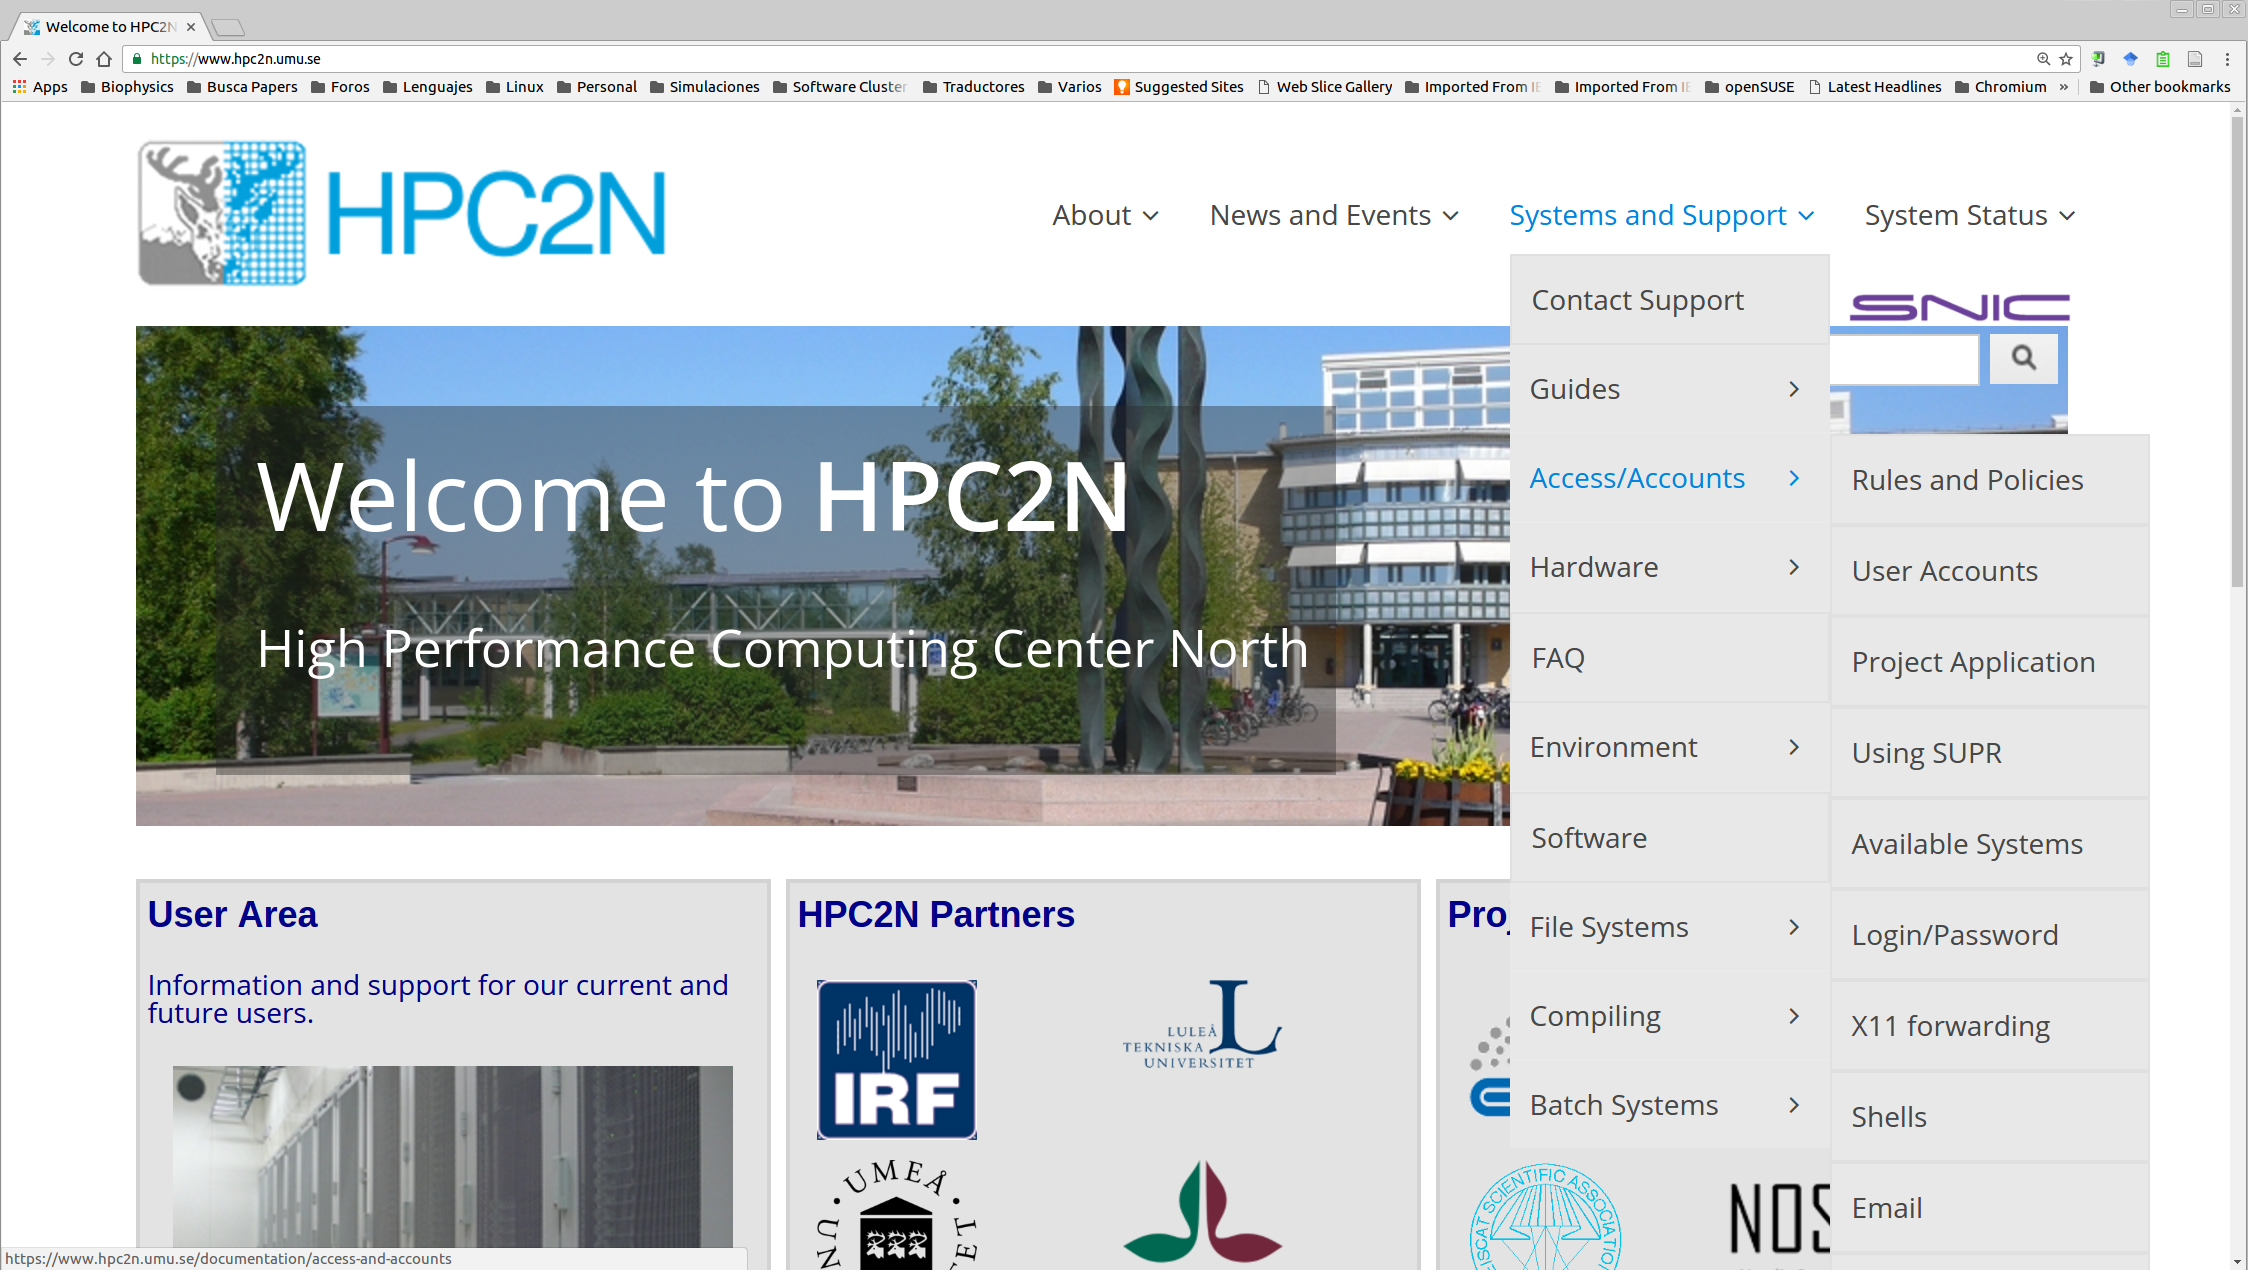
\includegraphics[width=10.5cm]{images/web.png}

\end{frame}

\begin{frame}
	\frametitle{User Support}

	\begin{itemize}
		\item	Meetings with individuals or groups
			\begin{itemize}
				\item	To see how can HPC2N be of help
				\item	Help to get started
				\item	Help to parallelize
			\end{itemize}
		\item	HPC2N Think Tank - Open house
		\item	Courses (0.5 - 3 days)
			\begin{itemize}
				\item	Introduction on how to use our system
				\item	Parallel programming (MPI, OpenMP) Oct. 2016
				\item	Computational Chemistry, MD simulations Nov. 2016
			\end{itemize}
	\end{itemize}

\end{frame}

